\section{Error Functions}\label{sec:error-functions}
Sometimes also called objective functions or loss-functions.

\subsection{Mean-Squared Error}\label{sec:mse}
As the name suggests the \gls{MSE} is defined as the mean (over all training examples) of squared difference between the correct value $t_i$ und the correct value $o_i$. This big errors are punished harder than small differences.
\begin{equation}\label{eq:mse}
E_{\text{MSE}} = \frac{1}{n} \sum_{i=1}^n (t_i - o_i)^2
\end{equation}
This would derive to
\begin{align}
\begin{split}
\frac{\partial E_{\text{MSE}}}{\partial o_j}
&= \frac{1}{n} \sum_{i=1}^n \frac{\partial (t_i - o_i)^2}{\partial o_j}\\
&= \frac{1}{n} \frac{\partial (t_j - o_j)^2}{\partial o_j}\\
&= \frac{1}{n} 2 (t_j - o_j) (-1)\\
&= \frac{2}{n} (o_j - t_j)
\end{split}
\end{align}
which is technically fine, but as the fraction is only a constant factor, we will often use a a slightly different definition:
\begin{align}\label{ed:mse2}
E_{\text{MSE}} &= \half \sum_{i=1}^k (t_i - o_i)^2\\
\frac{\partial E_{\text{MSE}}}{\partial o_j}
&= - (t_j - o_j) = o_j - t_j
\end{align}

\subsection{Cross Entropy Error}\label{sec:ce}
\Gls{CE} works great well on classifications tasks. $t_i$ is either $0$ or $1$ and $o_i$ is the class probability computed by the network $\Rightarrow o_i \in (0, 1]$ as $log(0)$ is not defined.
\begin{equation}\label{eq:ce}
E_{\text{CE}} = - \sum_{i=1}^k \left( t_i \log(o_i) + (1 - t_i) \log(1 - o_i) \right)
\end{equation}
This will derive to:
\begin{align}
\begin{split}
\frac{\partial E_{\text{CE}}}{\partial o_j} &= - \frac{\partial}{\partial o_j} \sum_{i=1}^k \left( t_i \log(o_i) + (1 - t_i) \log(1 - o_i) \right)\\
&= - \frac{\partial}{\partial o_j} t_j \log(o_j) - \frac{\partial}{\partial o_j} (1 - t_j) \log(1 - o_j)\\
&= - \frac{t_j}{o_j} + \frac{1 - t_j}{1 - o_j}\\
&= \frac{1 - t_j}{1 - o_j} - \frac{t_j}{o_j}
\end{split}
\end{align}

\begin{figure}
\centering
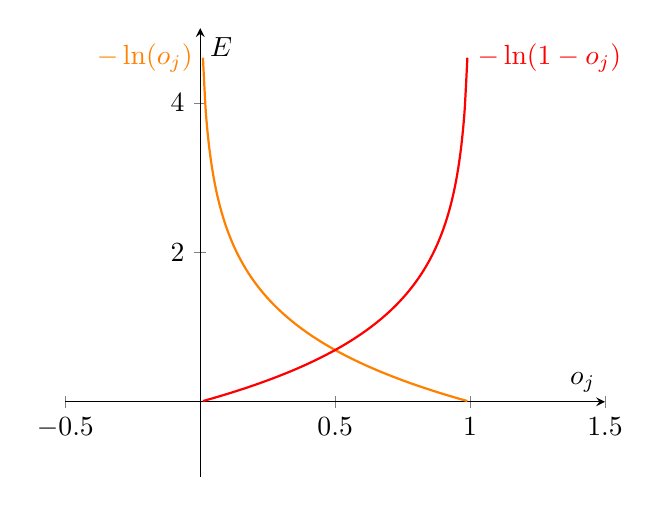
\begin{tikzpicture}
\begin{axis}[
	axis lines = middle,
	xlabel = $o_j$,
	ylabel = $E$,
	ymin = -1,
	ymax = 5,
	xmin = -0.5,
	xmax = 1.5,
	clip = false,
]
\addplot[
	domain = 0:0.99,
	samples = 100, 
	color = orange,
	thick, smooth,
	]
{-ln(x)}
node[left,pos=0] {$-\ln(o_j)$};
\addplot[
	domain = 0.01:1,
	samples = 100, 
	color = red,
	thick, smooth,
	]
{-ln(1-x)}
node[right,pos=1] {$-\ln(1-o_j)$};	
\end{axis}
\end{tikzpicture}
\caption{Error produced for $t_j=1$ (orange) and for $t_j=0$ (red). $o_j$ must be in range $(0,1]$, otherwise the logarithm can be complex or undefined or the error gets rediciously large.}
\end{figure}

\subsection{L1 and L2 Regularization}
Small weights tend to perform better and we can modify the error functions from above to penalize big weight by adding additional error terms.
\begin{itemize}
\item L1 norm: $||\mathbf{w}||_{L1} = \sum_j |\mathbf{w}_j|$
\item L2 norm: $||\mathbf{w}||_{L2} = \sum_j \mathbf{w}_j^2$
\item new error function $E' = E + \alpha_{L1} ||\mathbf{w}||_{L1} + \alpha_{L2} ||\mathbf{w}||_{L2}$
\item new hyperparamaters $\alpha_{L1}$ and $\alpha_{L2}$, optimize on development set
\end{itemize}
